% -*-latex-*-
% Document name: input.tex
% Creator: Rob MacLeod [macleod@cvrti.utah.edu]
% Last update: September 4, 2000 by Rob MacLeod
%    - created
% Last update: Sun Sep 24 22:22:21 2000 by Rob MacLeod
%    -  Version 5.0Beta release edition
% Last update: Thu Sep  7 12:37:00 2000 by Rob MacLeod
%    - first full version
% Last update: Mon Jul 23 13:28:30 2001 by Rob MacLeod
%    - release 5.2
% Last update: Fri Mar 1 20:00:00 2002 by Bryan Worthen
%    - release 5.3
% Last update: Fri Jun 21 13:24:14 2002 by robmacleod
%    - An update to align with 5.3 + recent changes
% Last update: Fri Jan 24 20:00:00 2003 by Bryan Worthen
%    - release 5.4
% Last update: Wed Oct 20 07:26:37 2004 by Rob Macleod
%    - release 6.2
% Last update: Wed Jan 31 07:26:37 2007 by Bryan Worthen
%    - release 6.4
% Last update: Fri Feb 16 08:20:52 2007 by Rob Macleod
%    - release 6.5
%%%%%%%%%%%%%%%%%%%%%%%%%%%%%%%%%%%%%%%%%%%%%%%%%%%%%%%%%%%%%%%%%%%%%%

%begin{latexonly}
  \newcommand{\indirec}%
  {\centerline{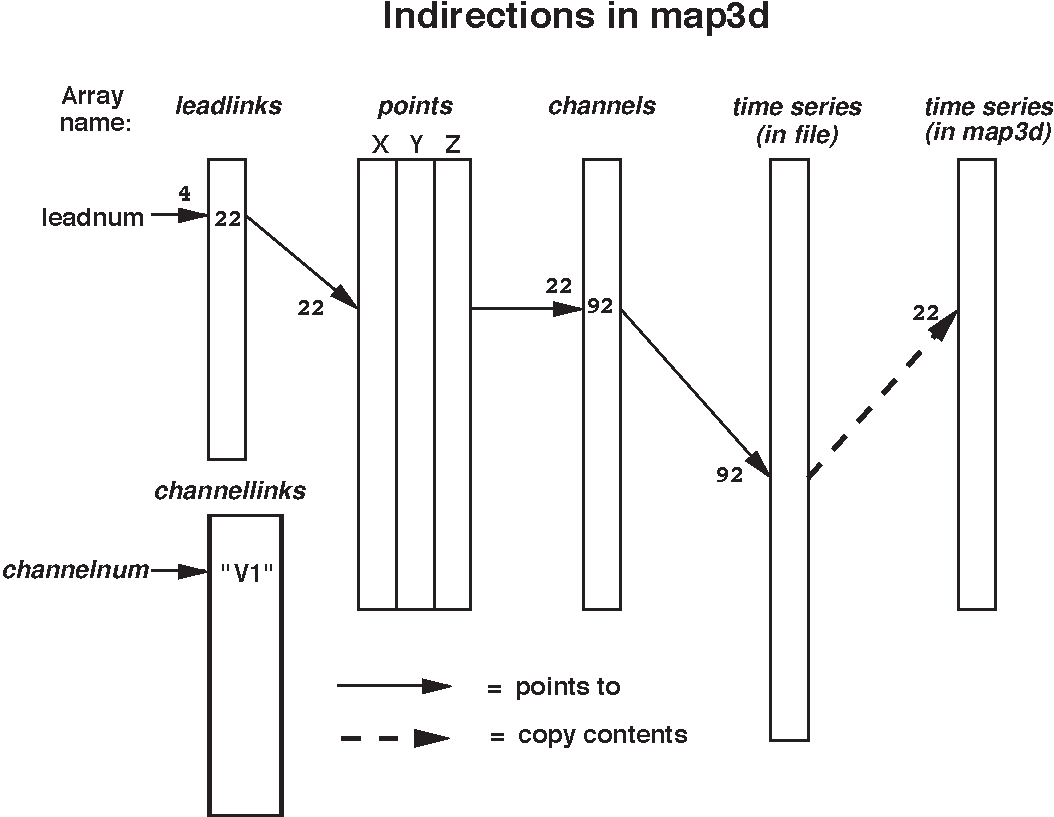
\includegraphics[width=4in] 
      {figures/map3d-indirection.pdf}}}
%end{latexonly}
\begin{htmlonly}
  \newcommand{\ethphoto}{%
     \htmladdimg[align=top,alt="indirection"]
                {figures/map3d-indirection.pdf}}
\end{htmlonly}


\section{Input files}

%% -*-latex-*-
% Document name: defaultfile.tex
% Creator: Rob MacLeod [macleod@cvrti.utah.edu]
% Last update: September 4, 2000 by Rob MacLeod
%    - created but not included in version 1.0 of the manual
%%%%%%%%%%%%%%%%%%%%%%%%%%%%%%%%%%%%%%%%%%%%%%%%%%%%%%%%%%%%%%%%%%%%%%
\subsection{Default settings files}
\label{sec:defaults} 

\map{} looks for files containing default settings for
many parameters that are relevant to the control of the program.
The order of precedence is as follows:
%
\begin{enumerate}
  \item The {\tt-df filename} option defines the file with highest
        precedence default settings.
  \item A file named {\tt .map3drc} in the current directory (the one from
        which the application was launched) is used next.
  \item If no {\tt .map3drc} files is found in the current directory, it is
        searched for in the user's home directory (see the HOME
        environmental variable).  This file has the lowest precedence and
        is only used of the other two options are not found.
  \item The program \map{} has a set of internal defaults which are used
        if there are no external default files found.
\end{enumerate}

\newpage
The format of the default file is as follows:
%
\begin{verbatim}
           # comment line (ignored by map3d)
           parameter = value
\end{verbatim}

\noindent
where the parameters and values are taken from the following list:

\begin{center}
\begin{tabular}{|l|l|p{3.2in}|} \hline
\multicolumn{1}{|c|}{Parameter} &
\multicolumn{1}{|c|}{Values} &
\multicolumn{1}{|c|}{Meaning} \\ \hline
shadingmodel & GOURAUD & Use Gouraud shading of triangles \\ 
             & FLAT    & Use flat shading of triangles \\ \hline
scale\_scope  & GLOBAL\_SURFACE & Scaling global over each surface \\ 
             & GLOBAL\_FRAME   & Scaling global over each frame of data \\
             & GLOBAL\_GLOBAL  & Scaling global over all data \\
             & LOCAL          & Scaling local to each frame and surface\\
             & USER           & Scaling by user-supplied values (-pl -ph)
             \\
\hline
scale\_model  & LINEAR & Use linear scaling of contours \\
             & LOG    & Use logarithmic scaling \\
             & EXP    & Use exponential scaling \\
             & LAB7   & Use logarithmic in 7 levels scaling \\
             & LAB13  & Use logarithmic in 13 levels scaling \\ 
\hline
scale\_mapping & SYMMETRIC & scale symmetrically around both side of zero\\
              & SEPARATE  & scale separately for + and - data values\\
              & TRUE\_MAP  & scale from most - to most + values\\
\hline
color\_map     & RG       & Use full red-to-green colour map \\
              & RG2      & Use red-and-green (2-colour) colour map \\
              & FULL     & Use blue-to-red (full) colour map \\
              & BTW      & Use black-to-white colour map \\
              & WTB      & Use white-to-black colour map \\
\hline
lead\_marking\footnotemark 
              & LEADS          & mark nodes with lead (channel)
                                                             numbers\\ 
              & NODES          & mark nodes with node numbers\\
              & VALUES         & mark leads with potential values\\
              & CUBES          & mark leads with spheres/cubes \\
              & MINMAX\_LABELS & mark extrema with lead numbers \\
              & MINMAX\_CUBES  & mark extrema with cubes \\
              & SCALAR         & mark the selected scalar node \\
\hline
num\_cols      & value    & number of colours to use in shade display\\ \hline
num\_conts     & value    & number of contour levels in display\\ \hline
draw\_bbox     & TRUE/FALSE & set bounding box on or off \\ \hline
datafile\_path & pathame  & alternate path to the .pak/.raw files 
in .tsdf file. \\ \hline
geomfile\_path & pathame  & alternate path to the .geom files 
in .tsdf file. \\ \hline
report\_level  & value    & level of error reporting ( 0--3 ) \\ \hline
\end{tabular}
\end{center}

\footnotetext{options are cumulative} 

Note that these parameters and values are not case sensitive and that they
can all be overridden during execution of the program, typically via the
mouse menu (right mouse button).  See section~\ref{sec:scaling} for details
on the different scaling options.  The list of parameters possible will
also certainly grow with the program.

To save the current settings in a file, there is an option in the main menu
of \map{} which dumps all the settings to the file {\tt ./.map3drc}, that
is, the file {\tt .map3drc} in the current directory.  That way, when you
start the program again from that directory, the same settings will be loaded.
The {\tt .map3drc} file is just a normal text file, but like all
``rc''-files, it is hidden from the {\tt ls} command unless you add the
{\tt -a} option (the alias {\tt la} is set up by default to do a long
listing of all files, including hidden files).  Dumping a copy of the
settings is also the easiest way to see what settings are currently being
maintained by \map{} and also forms the best starting point to setting up
your own customized default settings files.

 %?? Uncomment and update once this feature is working

In this section, we describe the contents and formats of all the input
files that \map{} uses to get geometry, data, and much more.

%%%%%%%%%%%%%%%%%%%%%%%%%%%%%%%%%%%%%%%%%%%%%%%%%%%%%%%%%%%%%%%%%%%%%%

\subsection{Geometry input files}
\label{sec:geomfiles} 

The input of geometric data for \map{} occurs via files and we support
three different formats at present.  The simplest (and oldest) is a set of
ASCII files that contain the points or nodes of the geometry---stored in a
file with the extension .pts---and the connectivities that described
polygonal links between nodes---stored as line segments (.seg files),
triangles (.fac files), and tetrahedra (.tetra files).  To satisfy a need
for more comprehensive and compact storage of geometry information, we have
developed a binary file format and created the \graphicsio{} library to
manage these files.  Finally, in recognition of the ubiquity of MATLAB, as
of version 6.1, there is support for reading .mat files, which have an
internal structure that included node and connectivity information.  Below,
we describe each of these files and how \map{} uses them.

\subsubsection{Points (.pts) file}

The characteristics of a .pts file are as follows:
%
\begin{enumerate}
  \item ASCII file, no special characters permitted;
  \item Each line contains one triplet, ordered as x, y, and z values; one
        or more spaces between values, which are assumed to be real, 
        floating point numbers; 
  \item Each line may also optionally contain a group number as a fourth 
        element (although at present, \map{} does not use this group
        information); 
  \item the order of points in the file is the implicit order of the nodes in
        the geometry; connectivities are based on this ordering.
\end{enumerate}


\subsubsection{Triangle (.fac) files}

The characteristics of a .fac file are as follows:
%
\begin{enumerate}
  \item ASCII file, no special characters permitted;
  \item Each line contains a triplet of integer values pointing to the
        nodes of the geometry.  \textbf{Node numbers begin at 1 not 0!};
  \item The order of triangle vertices (nodes) is not strictly controlled,
        however, it is recommended that order reflect a common convention
        in graphics---a counterclockwise sequence of vertices when viewed from
        the {\bf outside} of the triangle;
  \item Each line may contain an optional fourth values which is the group
        number for the triangle (not used by \map{});
  \item Order of triangles in the file is not meaningful except for
        internal bookkeeping; user will notice ordering only when a
        triangle is picked for interrogation.
\end{enumerate}

\subsubsection{Binary (.geom) geometry files}
\label{sec:geomfile}


At the \htmladdnormallink{CVRTI} {http://www.cvrti.utah.edu} we have
developed a binary file system for efficient storage of complex geometry
and associated attributes, a part of what we call the \graphicsio{}
library.  Extensive documentation of this format is available from \rob{}
(\htmladdnormallink{www.cvrti.utah.edu/\~{}macleod/docs}
{http://www.cvrti.utah.edu/~macleod/docs}).

Briefly, each \graphicsio{} geometry file contains one or more sets of
node locations and, optionally, connectivities for polygonal elements
composed from those nodes.  It is possible in \graphicsio{} files to
associate scalar, vector, and tensor values to nodes or elements, the
most relevant example of which are channel pointers, stored as a set of
scalar values associated with the nodes of the geometry.  Each 
\graphicsio{} geometry file can contain any number of sets of 
geometries, each with different nodes and connectivities.  A typical
example for \map{} would be a single .geom file that contains information
from multiple surfaces that we might want to display together.


\map{} is capable of reading surface geometry from either single surfaces
or from all surfaces contained in a multi-surface geometry file. 
Command line arguments controls the selection, as we describe in the next
section.

\subsubsection{MATLAB geometry file support}
\label{sec:matlabgeom}

\map{} can read .mat files generated by MATLAB as long as they are
organized according to the following guidelines:
\begin{enumerate}
  \item Each separate surface is either a structure (See 
    the MATLAB documentation for 
%\htmladdnormallink{cells}
%    {http://www.mathworks.com/access/helpdesk/help/techdoc/matlab_prog/ch_da37a.html#67323}
%    and  
    \htmladdnormallink{structures}
    {http://www.mathworks.com/access/helpdesk/help/techdoc/matlab\_prog/ch02\_d27.html\#88951}
     ).  To include multiple surfaces requires an array of
    structures.
  \item Within a surface structure, the following fields contain the
    geometry:
    \begin{itemize}
      \item \emph{.pts or .node} contains the node locations, usually in a
        $3 \times N$ array (although \map{} will check and accept either $3
        \times N$ or its transpose, $N \times 3$), where $N$ is the number
        of nodes.
      \item \emph{.fac or .face} contains the triangle connectivities,
        usually in a $3 \times M$ array (again, \map{} will accept the
        transpose)\, where $M$ is the number of triangles.
      \item \emph{.seg or .edge} contains the line segment connectivities,
      \item \emph{.tet, .tetra, or .cell} contains tetrahedral
        connectivities, and
      \item \emph{.channels} contains the channel information in a
        one-dimensional vector, in which each element of the vector points
        to the associated data channel.
    \end{itemize}
\end{enumerate}

To prepare a structured .mat file is very simple, for example using the
following commands:
%
\begin{verbatim}
     >> geom.pts = ptsarray;
     >> geom.fac = facarray;
     >> geom.channels = 100:164
     >> save mygeom.mat geom
\end{verbatim}
%
where \verb|ptsarray| is a $3 \times N$ array defined to contain the node
locations, \verb|facarray| is a $3 \times M$ array of triangle
connectivities, and \verb|mygeom.mat| is the name of the resulting .mat
file.   The channels information indicates that there are 64 nodes in the
geometry and they expect to get time signals from channels 100--164 of a
data file.  (See Section~\ref{sec:leadfiles} for more information on
channels. 

\subsubsection{Landmark geometry file support}
\label{sec:landmarkgeom}

\map{} can also read geometry from a landmark file 
(See Section~\ref{sec:lmfile} below), where you specify a series
of connected points and radii.  \map{} will automatically connect
and triangulate them, and will also associate scalar data with them.
Note that currently there is no channels support for landmark geometry.


%%%%%%%%%%%%%%%%%%%%%%%%%%%%%%%%%%%%%%%%%%%%%%%%%%%%%%%%%%%%%%%%%%%%%%

\subsection{Command line control of geometry files}
\label{sec:readgeom}


In \map{} the -f option determines in which files the geometry is to be
found.  Starting from the filename that follows -f, which may or may not
include a file extension, the program looks for all possible candidate
geometry files and queries the user for resolution of any ambiguities.
Thus, with the arguments {\tt map3d -f myfile}, \map3d{} looks for
\texttt{myfile.geom}, \texttt{myfile.mat}, \texttt{myfile.pts},
\texttt{myfile.fac}, \etc{} and tries to resolve things so that a valid
geometry description is found.  It is possible to direct this process by
typing the geometry filename with an extension according to the following
rules:
%
\begin{center}
\begin{tabular}{|l|p{4in}|} \hline
\multicolumn{1}{|c|}{Extension} &
\multicolumn{1}{|c|}{Effect} \\ \hline
none & look for files with the extensions .pts, .fac, .tetra, and .geom and
if an incompatible set are present (\eg{} both .pts and .geom), ask user
which to take \\ 
.pts & take only the .pts file and ignore any connectivity or .geom file \\
.fac & take .pts and .fac and ignore any .geom files present. \\
.geom & take the graphicsio geometry file and ignore any others present. \\
.mat & take the MATLAB file and ignore any others present. \\ \hline
\end{tabular}
\end{center}

A further way to read geometry into \map{} is to use the geometry filename
that can be optionally contained within the time series file (see
Section~\ref{sec:datafiles}) that contains the potentials.  This requires
that the .tsdf file be created with the geometry filename
included; adding this after the fact is difficult.  Note that even if a
geometry filename is found in the .tsdf file, it can be overridden
by the geometry file name specified in the argument list of \map{}.

%%%%%%%%%%%%%%%%%%%%%%%%%%%%%%%%%%%%%%%%%%%%%%%%%%%%%%%%%%%%%%%%%%%%%%

\subsection{Scalar data files}
\label{sec:datafiles} 

There are three ways of storing scalar values (typically electric potential
in our applications) so that \map{} can recognize and read them.  One is a
simple ASCII file, one is a binary format developed at the
CVRTI\@, and the third is MATLAB. 

\subsubsection{.pot files}
\label{sec:potfiles} 

One way to package the scalar data values that are assigned to the points
in the geometry is the .pot file.  In the default condition,
the scalar values in the .pot files are ordered in the same way as
the node points in the geometry file with simple one-to-one assignment.
With a channels file, it is possible to remap this assignment, as described
in Section~\ref{sec:leadfiles}).

\noindent
The rules for .pot files are:
%
\begin{enumerate}
  \item Each line of the files contains one scalar data value, assumed to
        be a real number in single precision floating point format. 
  \item The order of the values within the file must either agree with that
        of the associated set of nodes or a channels file must be supplied
        to redirect the links between potential value and nodes.
  \item Each .pot file {\em must\/} end with a blank line.
  \item A single .pot file can contain only the data values
        associated with a single surface at a single instant in time.  To
        represent a sequence of time steps (frames) requires a sequence of
        files, typically with filenames ending in a three-digit series,
        \eg{} \texttt{mapdata001.pot}, \texttt{mapdata002.pot},
        \texttt{mapdata003.pot}, \ldots{}.  Section~\ref{sec:scalarparams}
        explains how to specify such a series of .pot files to \map{} and
        Section~\ref{sec:usage-examples} shows examples.
  \item The extension .pot {\em must\/} be used.
\end{enumerate}


\subsubsection{CVRTI data (.tsdf and .tsdfc) format files}
\label{sec:tsdffile} 

One efficient and flexible way to store scalar values is by means of the
time-series data file format developed at the CVRTI, also as part of the
\graphicsio{} library.  Each time series data file (.tsdf files) holds an
entire sequence, or \emph{time series} of scalar data in a single file,
along with some information about the contents, type, units, and global
(\ie{} that apply to all channels) temporal fiducials from the time series.
For more details on this file format see
\htmladdnormallink{www.cvrti.utah.edu/\~{}macleod/docs/graphicsio}
{http://www.cvrti.utah.edu/~macleod/docs/graphicsio}.

Here are some concepts of the time series data file structure that are
relevant to the different modes of operation described in this manual.
%
\begin{description}
  \item [Links to geometry]  The
        links between the channels of data in the .tsdf file and the nodes
        of the surface[s] over which they are displayed is established via
        {\em channel\/} array information, which is available stored as
        associated scalars to the nodes in the geometry file (see
        Section~\ref{sec:geomfiles}) or in explicit channels files (see
        Section~\ref{sec:leadfiles}).
  \item [Frames]  By {\em frames\/} of data, we mean instants in the data
        stream representing single moments in time.  For each frame, there
        is a set of values that for a spatial distribution or map and
        \map{} needs to know what subset of frames are to be 
        included in the display.  To explicitly specify frame numbers, use
        the \texttt{-s} and \texttt{-i} options described in
        Section~\ref{sec:usage}.  As an example, the command line
\begin{verbatim}
        map3d -w -f geomfile.geom@1 -p datafile.tsdf -s 10 130 -i 2
\end{verbatim}
        specifies that surface 1 from the geometry file {\tt geomfile.geom}
        should be used to display frames 10 to 130, taking every second
        frame, from run 2 of the time series data file {\tt datafile.tsdf}.
\end{description}


\paragraph{Time series container files (tsdfc): } 
\label{sec:tsdfcfile}

There is an extension to the \graphicsio{} library that defines a container
file format for a set of time series data (.tsdf) files, and
can contain parameters extracted from the associated time series.  These
files are actually small databases and we use a modified (patched actually)
version of the GNU Database Library (GDBL) to manage them.  

Examples of programs and libraries that provide support for .tsdfc
files include Everett, a program by Ted Dustman for initial processing of
mapping data,  \htmladdnormallink{Matmap}
{http://www.cvrti.utah.edu/~jeroen/matmap/}, a set of MATLAB uilities by
Jeroen Stinstra with a similar functionality, and \texttt{tsdflib} (as yet
undocumented), a library created by Ted Dustman, Rob MacLeod, Jenny
Simpons, and Jeroen Stinstra that provides C-language access to container
files.

For more information on container files, see the documentation for the
graphicsio library at
\htmladdnormallink{www.cvrti.utah.edu/\~{}macleod/docs/graphicsio/}
{http://www.cvrti.utah.edu/~macleod/docs/graphicsio/}. 

\subsubsection{MATLAB data file support}
\label{sec:matlabdata}

You can also store and read scalar values in .mat files, as a structure
with a single field called ``.potvals'', that contains a $N \times M$ array,
where $N$ is the number of data channels and $M$ is the number of time
instants.  There are additional fields in the structure that mimic the
information available in the graphicsio .tsdf file so---the complete list is
as follows:
%
\begin{itemize}
  \item \emph{.potvals, .data, .field, or .scalarfield} scalar values as $N
    \times M$ array, where $N$ is the number of data channels and $M$ is
    the number of time instants.
  \item \emph{.unit} the type of units for the data, ``um'' for microvolts,
  ``mv'' for millivolts and ``V'' for volts.
  \item \emph{.label} the name of the time series.  This is optional, but is
    useful in identifying the time series, particularly from a 
    multi-time-series file.
  \item \emph{.fids} a structure (or array of structures) containing
    fiducial time markers for the time series (see below for details of
    fidicual storage).
\end{itemize}

Note that only the 'potvals' field is required.  A matlab array may 
be one instance of these fields, a cell or struct array of them, or 
simply an $N \times M$ array of data.  To read a matlab file with many time
time series, specify the time series on the command line with the '@' symbol
(See Section~\ref{sec:scalarparams}) or specify the time series in the 
file browser.  It will be shown by the label specified in the matlab file.

The commands to make a suitable .mat file are very easy in MATLAB, for
example, to load 128 channels of time signals with unit of millivolt from
an array \texttt{sockinfo} in MATLAB to a file called
\texttt{mysockdata.mat}
%
\begin{verbatim}
    >> sockdata.potvals   = sockinfo(1:128,:);
    >> sockdata.unit = 'mV'
    >> sockdata.lavel = 'A set of cool sock data'
    >> save mysockdata.mat sockdata
\end{verbatim}

\subsubsection{Fiducial (ascii) files}
\label{sec:fidfiles}

A fiducial can be input currently also in three ways: via a .tsdfc file,
where the potential and fiducial values are stored together, via a .fids
file, a simple ASCII file containing the values for each node, or by means
of the MATLAB file that contains the time series data.

\paragraph{MATLAB file format for fiducials}


The fiducial information in a MATLAB time series data file is stored in a
array of structures called fids, where each element of the array represents
one set of fiducials.  This way, for example, there can be a set of $N$
activation times, another set of $N$ recovery times, and a set of $N$
Q-onset times.  Each element of the array is, in itself, a structure, so
that the set of fiducials contains enough information for \map{} to do a
useful display. 

The legal elements of a fids structure are as follows:
%
\begin{itemize}
  \item \emph{.type} the type of fiducial (see table below).
  \item \emph{.value} the array of fiducial values, one for each 
    channel of the data file.
\end{itemize}


Here is an example of creating the structures for some fiducials in MATLAB:
%
\begin{verbatim}
   matdata.potvals = potvals;
   matdata.unit = unit;
   matdata.label = label;
   matdata.fids(1).type = 10
   matdata.fids(1).value = fidvals(:,1);
   matdata.fids(2).type = 13;
   matdata.fids(2).value = fidvals(:,2);
   save (outfilename, 'matdata');
\end{verbatim}

The first three lines set up the time series data, as we have seen above.
The lines 4 and 5 create a set of fiducials of type 10 and loads the values
into that part of the data structure.  Lines 6 and 7 do the same thing for
a second set of fiducials, which have type 13. The final line saves the
contents of the structure into a file.

The type value for fiducials is important as \map{} associates colors to
fiducial types to provide consistent display.  Moreover, each type has an
associated text label that \map{} uses in the interface.  The list of
current fiducial types and their numbers is as follows:

\bigskip

\begin{center}
\begin{tabular}[h]{|c|l|} \hline
\multicolumn{2}{|c|}{Fiducial Types} \\  \hline \hline
Number & Type \\ \hline 
 0 & pon, pstart \\
 1 & poff, pend \\
 2 & qon, qrsstart, qrson \\
 3 & rpeak, qrspeak \\
 4 & soff, qrsend, qrsoff \\
 5 & stoff, tstart, ton \\
 6 & tpeak \\
 7 & toff \\
 8 & actplus \\
 9 & actminus \\
 10 & act \\
 11 & recplus \\
 12 & recminus \\
 13 & rec \\
 14 & ref, reference \\
 15 & jpt, jpoint \\
 16 & baseline \\
 30 & pacing \\
\hline
\end{tabular}
\end{center}

\paragraph{ASCII file format for fiducials}

The characteristics of a .fids file are as follows:
\begin{enumerate}
  \item ASCII file
  \item must have the following at the top of the file, on each line:
  \begin{enumerate}
    \item number of time series, e.g., 1 (\map{} only allows 1)
    \item series number (space) pak number
    \item number of nodes (space) list of fiducial types
  \end{enumerate}
  \item each successive line contains the node number followed by
        a list of fiducial values, one corresponding to each
        type specified on the line with the node numbers
\end{enumerate}

\begin{verbatim}
    Example:
    1
    1 -1
    256 activation recovery
    1 8 212
    2 16 225
    3 9 214
    ...
    255 39 248
    256 25 237  
\end{verbatim}


%%%%%%%%%%%%%%%%%%%%%%%%%%%%%%%%%%%%%%%%%%%%%%%%%%%%%%%%%%%%%%%%%%%%%%

\subsection{Channels and leadlinks}
\label{sec:leadfiles} 

\subsubsection{Description of leadlinks and channels
information}

Channels and leadlinks files, and the arrays they
contain, are identical in structure, but they have important {\bf
functional differences}.  A run of \map{} may require both, either, or
neither of these, depending on the structure of the data files and
geometries. The basic function of both channels and leadlinks information
is to offer linkages between nodes in the geometry and the data that is to
be associated with those nodes.  The first file type, the channels file,
links the nodes in the geometry to specific time signals in a data file;
without channel mapping, the only possible assumption is that each node $i$
in the geometry corresponds to the same time signal $i$ in the data file.
Any other linkage of geometry and data channel requires there to be channel
information, typically either from a separate .channels file or stored with
the binary .geom file as an associated scalar value for each node.

\begin{figure}[htb]
   \begin{makeimage}
    \end{makeimage}
    \indirec
    \caption{\label{fig:indirec}Example of the indirection possible in
      \map{} through the use of {\em leadlinks\/} {\em channels}, and {\em
        channellinks}.  Lead number 4 points, via the {\em leadlinks\/}
      array to node number 22.  This, in turn, points via the {\em
        channels\/} array to location 92 in the multiplexed data buffer,
      which causes the values at time signal 92 to be loaded into location
      22 in the internal data array (and displayed by \map{}).  In a
      separate, \emph{channellinks} array, shown below the leadlinks array,
      the entry in lead 4 says that that lead should actually be labeled
      ``${\rm V_{1}}$''. }
\end{figure}

Leadlinks are purely for visualization and describe the connection between
``leads'', a measurement concept, with ``nodes'', a geometric location in
space.  In electrocardiography, for example, a lead is the algebraic
difference between two measured potentials, one of which is the reference;
``unipolar'' leads have a reference composed of the sum of the limb
electrode potentials.  It is often useful to mark the locations of these
leads on the geometry, which often contains many more nodes than there are
leads.  The most frequent use to date has been to mark the locations of the
standard precordial ECG leads within the context of high resolution body
surface mapping that uses from 32--192 electrodes.  Another common
application is to mark subsets of a geometry that correspond to 
measurement sites (values at the remaining nodes are typically the product
of interpolation).  In summary, leadlinks allow \map{} to mark specific
nodes that may have special meaning to the observer.

Figure~\ref{fig:indirec} shows an example of lead and channels
information and their effect on \map{}.  See the figure caption for
details. 


\map{} handles this information in the following manner:
%
\begin{description}
  \item [channels]  The {\em channels\/} information links 
        nodes in the geometry to individual channels or time series in the
        data file.  For example, the data values associated with node
        $k$ in the geometry are located in the data location specified by
        the channel array value ${\rm channels}(k)$.  If ${\rm channels}(k)
        < 0$, then there is no valid data for node $k$.

        Note that \textbf{ \map{} uses the channels arrays when
        loading scalar data into the internal storage arrays!}  Hence, the
        action of the channel mapping is not reversible.   Should geometry
        nodes and data channels match one-to-one, there is no need for a
        channels array.  It is also possible to define via a channels array
        the situation in which a single data channel belongs to two (or
        more) nodes in the geometry.  The most frequent example of this
        occurs when three-dimensional geometries are ``unwrapped'' into
        surfaces in which what was a single edge is split and thus present
        at both ends of the surface.

  \item [leadlinks] The {\em leadlinks\/} information is primarily
        used to identify and mark measurement lead specific within the
        geometry.  The typical use is to select a subset of the nodes to
        identify the measurement sites---values at other sites might
        be interpolated or otherwise computed.  Leadlinks also provide a
        means to renumber the labels on the nodes of the geometry in order
        to, for example, reproduce the numbering scheme used in an
        experimental setup.
        
        In the leadlinks array each entry refers, by its location in the
        array, to a particular lead \#; the value at that location in the
        array gives the number of the node in the geometry file to be
        associated with this lead.  For example if lead 4 has a leadlinks
        entry of 22 (${\rm leadlinks}(4)=22$), then \map{} will display
        node 22 in the geometry as ``4'', not ``22'' whenever node marking
        with \emph{leads} is selected).

  \item [channellinks] There is an extension of the basic scheme which
        includes a further level of redirection for giving the leads
        explicit text labels.  Channel links are stored as a array of
        strings, one for each node of the geometry.  The channellinks file
        is organized similarly to a leadlinks file, with each line
        containing information for one node.  However, each line consists
        of two values, 1) the number of the associated channel and 2) the
        text string to be used as the label when \map{} marks the nodes
        with channel numbers.
        
        Hence we have the situation of a node number $K$ in the geometry 
        displaying time signals from channel $L$ in the scalar data, but
        labeled with string ``XXX''. 

\end{description}

\subsubsection{Source of leadlink and channel information}

The sources of channels, leadlinks, and channellinks information are
files, or parts of files, as outlined in the following paragraphs.

\paragraph{In .geom files}

Information for the {\em channels\/} array is stored as an associated
scalar with the information in the standard .geom files.  At
present, there is no leadlinks array stored in the .geom file but
this could change in the future.

\paragraph{In .mat geometry files}

MATLAB geometry files can also contain an {\em channels\/} array is stored as
a .channels field in the structure.  See Section~\ref{sec:matlabgeom} for
more details.


\paragraph{In .leadlinks files}

A .leadlinks file is an ASCII file, the first record of which
contains a line {\tt nnn leads}, where {\tt nnn} is the number of leads to
be described in the file (and also one less than the total number of lines
in the file).  Each following record contains two integer values:\\
%
\begin{enumerate}
  \item the first number is the number of the lead, as it should appear in
        any labeling of the associated node.
  \item the second entry in each row is the value of the associated node
        number in the geometry.  
 \end{enumerate}
%
For example, the file for a surface which reads:
%
\begin{verbatim}
    32 Leads
    1   1   
    2   42  
    4   31  
    7   65  
    .   .   
    .   .   
    .   .   
    32  11     <---- 32nd entry in the file, at line 33 of the file.
\end{verbatim}
%
indicates that there are 32 leads to be linked (the geometry can, often
does, contain more than 32 nodes), and that lead \#1 is called lead ``1''
and is node 1 in the geometry file.  Lead \#2 is at node 42, lead \#3 is
called ``4'' and is found at node 31.  Likewise, lead \#4 is called ``7'',
and is located at node 65, and so on, up to lead \#32, called ``32'', at
node 11.

Nodes listed in a {\em leadlinks} file that is passed to \map{} with the
{\tt -ll} option can be marked in a number of ways, described more fully in
Table~\ref{table:nodemarking} in Section~\ref{sec:control-menus}.

\paragraph{In .channels files}

A \emph{channels} file is an ASCII file, the first record of which contain a
line {\tt nnn nodes}, where {\tt nnn} is the number of nodes to be
described in the file (and also one less than the total number of lines in
the file).  There is one line in the file for each node of the geometry to
which we wish to associate scalar data.   Each following record contains
two integer values:\\ 
%
\begin{enumerate}
  \item the first number is simply a running counter that indicates
        the node number with which to associated the second value in the
        row.
  \item The second value in each row is the {\em channel\/} number for
        that node; a negative number signifies a node to which there is no
        data associated.
\end{enumerate}

\noindent
For example, the file for a surface which reads:
%
\begin{verbatim}
    352 Nodes
    1    123
    2    632
    .    .
    .    .
    22   -1
    23   432
    .    .
    .    .
    352  12
\end{verbatim}
%
indicates that there are 352 leads to be linked, and that the data value
for the first node is located at location 123 of the data file.  For node
2, the data value is to be found at location 632, and so on.  Node 22 does
not have any scalar data associated with it.

\subsubsection{Display of lead/channel information}

To see how \map{} can display the node and lead information, see
Sections~\ref{sec:displayleads} and~\ref{sec:control}. 

%%%%%%%%%%%%%%%%%%%%%%%%%%%%%%%%%%%%%%%%%%%%%%%%%%%%%%%%%%%%%%%%%%%%%%

  \subsection{Landmark files}
  \label{sec:lmfile} 

  Landmark files contain information for visual cues or landmarks that \map{}
  can draw over the surfaces in order to aid and orient the viewer. Initial
  use was primarily for coronary arteries, but the idea has expanded to
  incorporate a number of different orientation landmarks.  The original
  coronary artery class of landmarks requires only that each can be described
  as a series of connected points, with a radius defined for each point.  The
  coronary landmark is then displayed as a faceted ``pipe'' linearly
  connecting the points at the centre, with a radius, also linearly
  interpolated between points, determining the size of the pipe.  The
  landmark file can contain numerous, individual segments of such pipe-work,
  each of which is drawn separately.

  Other classes of landmarks are described below, but all of them can be
  described in a file with the following general format:
  %
  \begin{center}
  \begin{tabular}{|l|l|p{3.0in}|}
  \hline
  \multicolumn{1}{|c|}{Line number} &
  \multicolumn{1}{|c|}{Contents} &
  \multicolumn{1}{|c|}{Comments} \\ \hline
  1 & nsegs   & number of landmark segments in the file \\ \hline
  2 & 1 type nsegpts [segindex] [segcolor] & segment number (1), type, number of
  points, with optional index number and color (color is a RGB triple, 0-255 each) \\ 
  3 & X, Y, Z, radius [label] & point location and radius of point 1, with optional label to be drawn at the point \\
  4 & X, Y, Z, radius [label] & point location and radius of point 2 \\
  . & . & . \\
  . & . & . \\
  nsegpts + 2 & X, Y, Z, radius & point location and radius of last point in
                              segment 1 \\ \hline
  . & 2 type nsegpts [segindex] [segcolor] & segment number (2), type, number of
  points, with optional index number and color \\ 
  . & X, Y, Z, radius [label] & point location and radius of point 1 \\
  . & X, Y, Z, radius [label] & point location and radius of point 2 \\
  . & . & . \\
  . & . & . \\
  . & X, Y, Z, radius [label] & point location and radius of last point in
                              segment 2 \\ \hline
  . & . & . \\
  . & . & . \\
  . & . & . \\
  . & . & . \\
  \hline
  \end{tabular}
  \end{center}

  The landmark types defined to date are the following:
  %
  \begin{center}
  \begin{tabular}{|l|p{1.5in}|p{3.5in}|} \hline
  \multicolumn{1}{|c|}{Name} &
  \multicolumn{1}{|c|}{Graph. object} &
  \multicolumn{1}{|c|}{Description}\\ \hline
  Artery & faceted pipe & a coronary artery/vein segment\\
  Occlusion & coloured sphere & an experimental occlusion that could be open and
  closed \\ 
  Closure & coloured sphere & a permanent occlusion that cannot be opened \\
  Stimulus & coloured sphere & a stimulus site \\
  Lead & coloured sphere & a particular electrode or lead location \\
  Plane & rectangular parallolopiped & a visible (but not functional) cutting
  plane through  the geometry (Note: do not confuse this with the cutting
  planes that \map{} provides for slicing through the  geometry).\\
  Rod & lines & rod inserted into needle track to digitize needle electrode
  locations. \\
  PaceNeedle & sphere & location of a pacing needle entry point\\
  Cath & faceted pipe & location of catheter in a vessel \\
  Fiber & arrow & local fiber direction indicator\\
  RecNeedle & sphere & location of recording needle entry point \\
  Cannula & tube & coronary vessel cannulus \\
  \hline
  \end{tabular}
  \end{center}

  Specifying  snare, closure, and stimulus requires a single point in the
  landmarks file, and the resulting sphere is coloured according to a set of
  values defined in the drawsurflmarks.c routine.  At present, the values
  used are:
  %
  \begin{center}
  \begin{tabular}{|ll|} \hline
    Occlusion & cyan \\ 
    Closure & blue \\
    Stimulus & yellow \\ \hline
  \end{tabular}
  \end{center}

  %
  and they are adjustable by the user, either via the Landmark menu, or by
  specifying a color for the segment

  To specify a plane landmark requires three ``points''
  %
  \begin{center}
  \begin{tabular}{|c|l|l|} \hline
    \multicolumn{1}{|c|}{Point} &
    \multicolumn{1}{|c|}{X,Y,Z} &
    \multicolumn{1}{|c|}{Radius} \\ \hline
  1 & First point of plane & Radius of the plane \\
  2 & Second point of plane & Thickness of the plane \\
  3 & Third point of plane & not used \\ \hline
  \end{tabular}
  \end{center}
  %
  The plane is drawn as a polygon with the number of sides controlled by a
  program variable. 

\paragraph{Filename conventions: } The standard extension of a
  landmark file is {\tt .lmarks} and the filename is specified by the {\tt
  -lm} parameter for each surface.

\paragraph{Control of landmark display: } for details of how to control the
display of landmarks, see Section~\ref{sec:control-landmarks}.



%%% Local Variables: 
%%% mode: latex
%%% TeX-master: "manual"
%%% End: 
